% Copyright (c) 2013 Joost van Zwieten

% Permission is hereby granted, free of charge, to any person obtaining a copy
% of this software and associated documentation files (the "Software"), to deal
% in the Software without restriction, including without limitation the rights
% to use, copy, modify, merge, publish, distribute, sublicense, and/or sell
% copies of the Software, and to permit persons to whom the Software is
% furnished to do so, subject to the following conditions:

% The above copyright notice and this permission notice shall be included in
% all copies or substantial portions of the Software.

% THE SOFTWARE IS PROVIDED "AS IS", WITHOUT WARRANTY OF ANY KIND, EXPRESS OR
% IMPLIED, INCLUDING BUT NOT LIMITED TO THE WARRANTIES OF MERCHANTABILITY,
% FITNESS FOR A PARTICULAR PURPOSE AND NONINFRINGEMENT. IN NO EVENT SHALL THE
% AUTHORS OR COPYRIGHT HOLDERS BE LIABLE FOR ANY CLAIM, DAMAGES OR OTHER
% LIABILITY, WHETHER IN AN ACTION OF CONTRACT, TORT OR OTHERWISE, ARISING FROM,
% OUT OF OR IN CONNECTION WITH THE SOFTWARE OR THE USE OR OTHER DEALINGS IN
% THE SOFTWARE.
%
\documentclass{tudelftposter}

% optional, makes QR code clickable
\usepackage[implicit=false,bookmarks=false]{hyperref}
\usepackage[utf8]{inputenc} % allow utf-8 input
\usepackage[T1]{fontenc}    % use 8-bit T1 fonts
\usepackage{url}            % simple URL typesetting
\usepackage{booktabs}       % professional-quality tables
\usepackage{amsfonts}       % blackboard math symbols
\usepackage{nicefrac}       % compact symbols for 1/2, etc.
\usepackage{microtype}      % microtypography
\usepackage{lipsum}
\usepackage{listings}
\usepackage{amsmath}
\usepackage{diagbox}
\usepackage{tabularx}
\usepackage{longtable}
\lstset{language = C}
\usepackage{graphicx,changepage}
\usepackage{float}
\usepackage{graphicx}
\usepackage{kotex}
\usepackage{xcolor}
\usepackage{color}
\usepackage{caption}
\usepackage{minted}
\usepackage{svg}
\usepackage{cclicenses}
\usepackage{tikz}
\usetikzlibrary{positioning}

\definecolor{mybluei}{RGB}{124,156,205}
\definecolor{myblueii}{RGB}{73,121,193}
\definecolor{mygreen}{RGB}{202,217,126}
\pgfdeclarelayer{background}
\pgfsetlayers{background,main}


\usepackage{setspace}

\hypersetup{%
  colorlinks=true,% hyperlinks will be black
  linkbordercolor=red,% hyperlink borders will be red
  pdfborderstyle={/S/U/W 2}% border style will be underline of width 1pt
}


\doublespacing
\graphicspath{./img/}
\title{마인크래프트 강화학습 환경 구축을 통한 멀티모달 연구\\
\large 와 특정 태스크에서의 우수성 비교}

\addauthornote{mail}[@]{\ttfamily yhs0602@snu.ac.kr}
% \addauthornote{diam}{Delft Institute of Applied Mathematics, TU Delft}
% \addauthornote{tp}{Department of Theoretical Physics, TU Delft}

% \addauthor[mail,diam]{J.F. Nash}
% \addauthor[diam,tp]{C.F. Gau{\ss}}
\addauthor{2019-13674 양현서 / 지도교수 장병탁}
% \addauthor[tp]{R.P. Feynman}

% \addfootimage(c:right column.center)[Delft Institute of Applied Mathematics]{tudelft}
% \ifqrcodessupported
%   % NOTE: compile this document with lualatex instead of pdflatex
%   \addfootqrcode(l:left column.left)[tudelft-poster repository]{http://github.com/joostvanzwieten/tudelft-poster}
% \else
%   \addfootobject*(l:left column.left)[research web page]{%
%     \begin{tikzpicture}
%       \node[red,draw,inner sep=1ex] {%
%         \begin{minipage}{15cm}
%           \footnotesize%
%           Please compile this document with lualatex to see a QR code here:\\
%           \null\texttt{\quad lualatex \jobname}
%         \end{minipage}};
%     \end{tikzpicture}}
% \fi

\begin{document}

% \SetSerifFonts{gt}{gt}
% \SetSansFonts{mj}{mj}
\section{서론}
\subsection{연구 주제}
강화학습을 위한 마인크래프트 환경에서 어둠 상태 효과를 활용한 시야 제한 태스크와 멀티모달 정보 활용의 중요성

\subsection{연구 동기 및 목적}
강화학습 에이전트들은 Atari 게임 등에서 높은 성능을 보였다. 하지만 이러한 문제들은 특정 도메인에 한정되어 있고, 다양한 입력 모드를 받지 않는다는 한계가 있다. 따라서, 다양한 도메인과 입력 모드를 포함하는 새로운 강화학습 환경의 구축이 필요하다. 이를 위해 마인크래프트를 활용할 수 있다. 마인크래프트는 다양한 상황과 조건을 가지고 있어 강화학습 알고리즘의 적용과 실험에 적합하다. 이렇게 마인크래프트를 강화학습 알고리즘 환경으로 활용한 관련 연구로는 MineDojo, MineRL 등이 있다. 그러나 이러한 환경들은 오래된 모드 프레임워크인 Forge를 사용하여 업데이트가 느리며, MineDojo는 마인크래프트 1.11.2 버전까지만 지원된다. 마인크래프트 1.19에는 "어둠(Darkness)" 상태 효과가 등장했다. 이는 플레이어의 시야를 좁게 만드는 상태 효과로, 새로운 도전 요소를 제공한다. 본 연구에서는 기존 연구들에서 지원하지 않은 최신 버전의 마인크래프트 환경의 어둠 상태 효과를 활용하여 현실의 야간 작업 등 시야가 제한된 상태에서의 태스크들을 제시하고, 기존 비전 기반 모델이 기존 환경에서 보이던 성능과 비교한다. 또한 기존 연구들에서 사용되지 않은 소리 정보를 활용하는 에이전트를 실험하여 멀티모달 정보 활용의 중요성을 강조하고 이를 통한 성능 향상을 확인할 것이다. 이러한 연구는 강화학습 알고리즘의 발전과 실제 응용에 새로운 통찰을 제공할 것으로 기대된다.

\section{이론적 배경}
\subsection{강화학습}
강화학습은 에이전트가 환경과 상호작용하며, 보상을 최대화하는 행동을 학습하는 방법이다. 강화학습은 다음과 같은 특징을 가진다.
\begin{itemize}
  \item 보상을 최대화하는 행동을 학습한다.
  \item 지도학습과 달리 데이터에 대한 레이블이 필요하지 않다.
  \item 시간 순서에 따라 행동을 수행하며, 이전의 행동이 다음 행동에 영향을 준다.
  \item 행동을 수행하고, 그에 따른 보상을 받는다.
\end{itemize}
강화학습 에이전트가 학습하기 위해 수집하는 정보가 에이전트의 행동에 종속적인 경향이 있어, 학습이 어렵다. 이러한 문제를 해결하기 위해 다양한 강화학습 알고리즘이 제안되었다. 본 연구에서는 강화학습 알고리즘 중 하나인 DQN을 사용한다.

\section{연구 방법}
\subsection{Environment}
Minecraft를 인간이 아닌 프로그램으로 조작하기 위해서 ``모드''라는 기능을 활용하였다. 모드를 이용하면 게임을 수정할 수 있다.

\begin{figure}
  \centering
  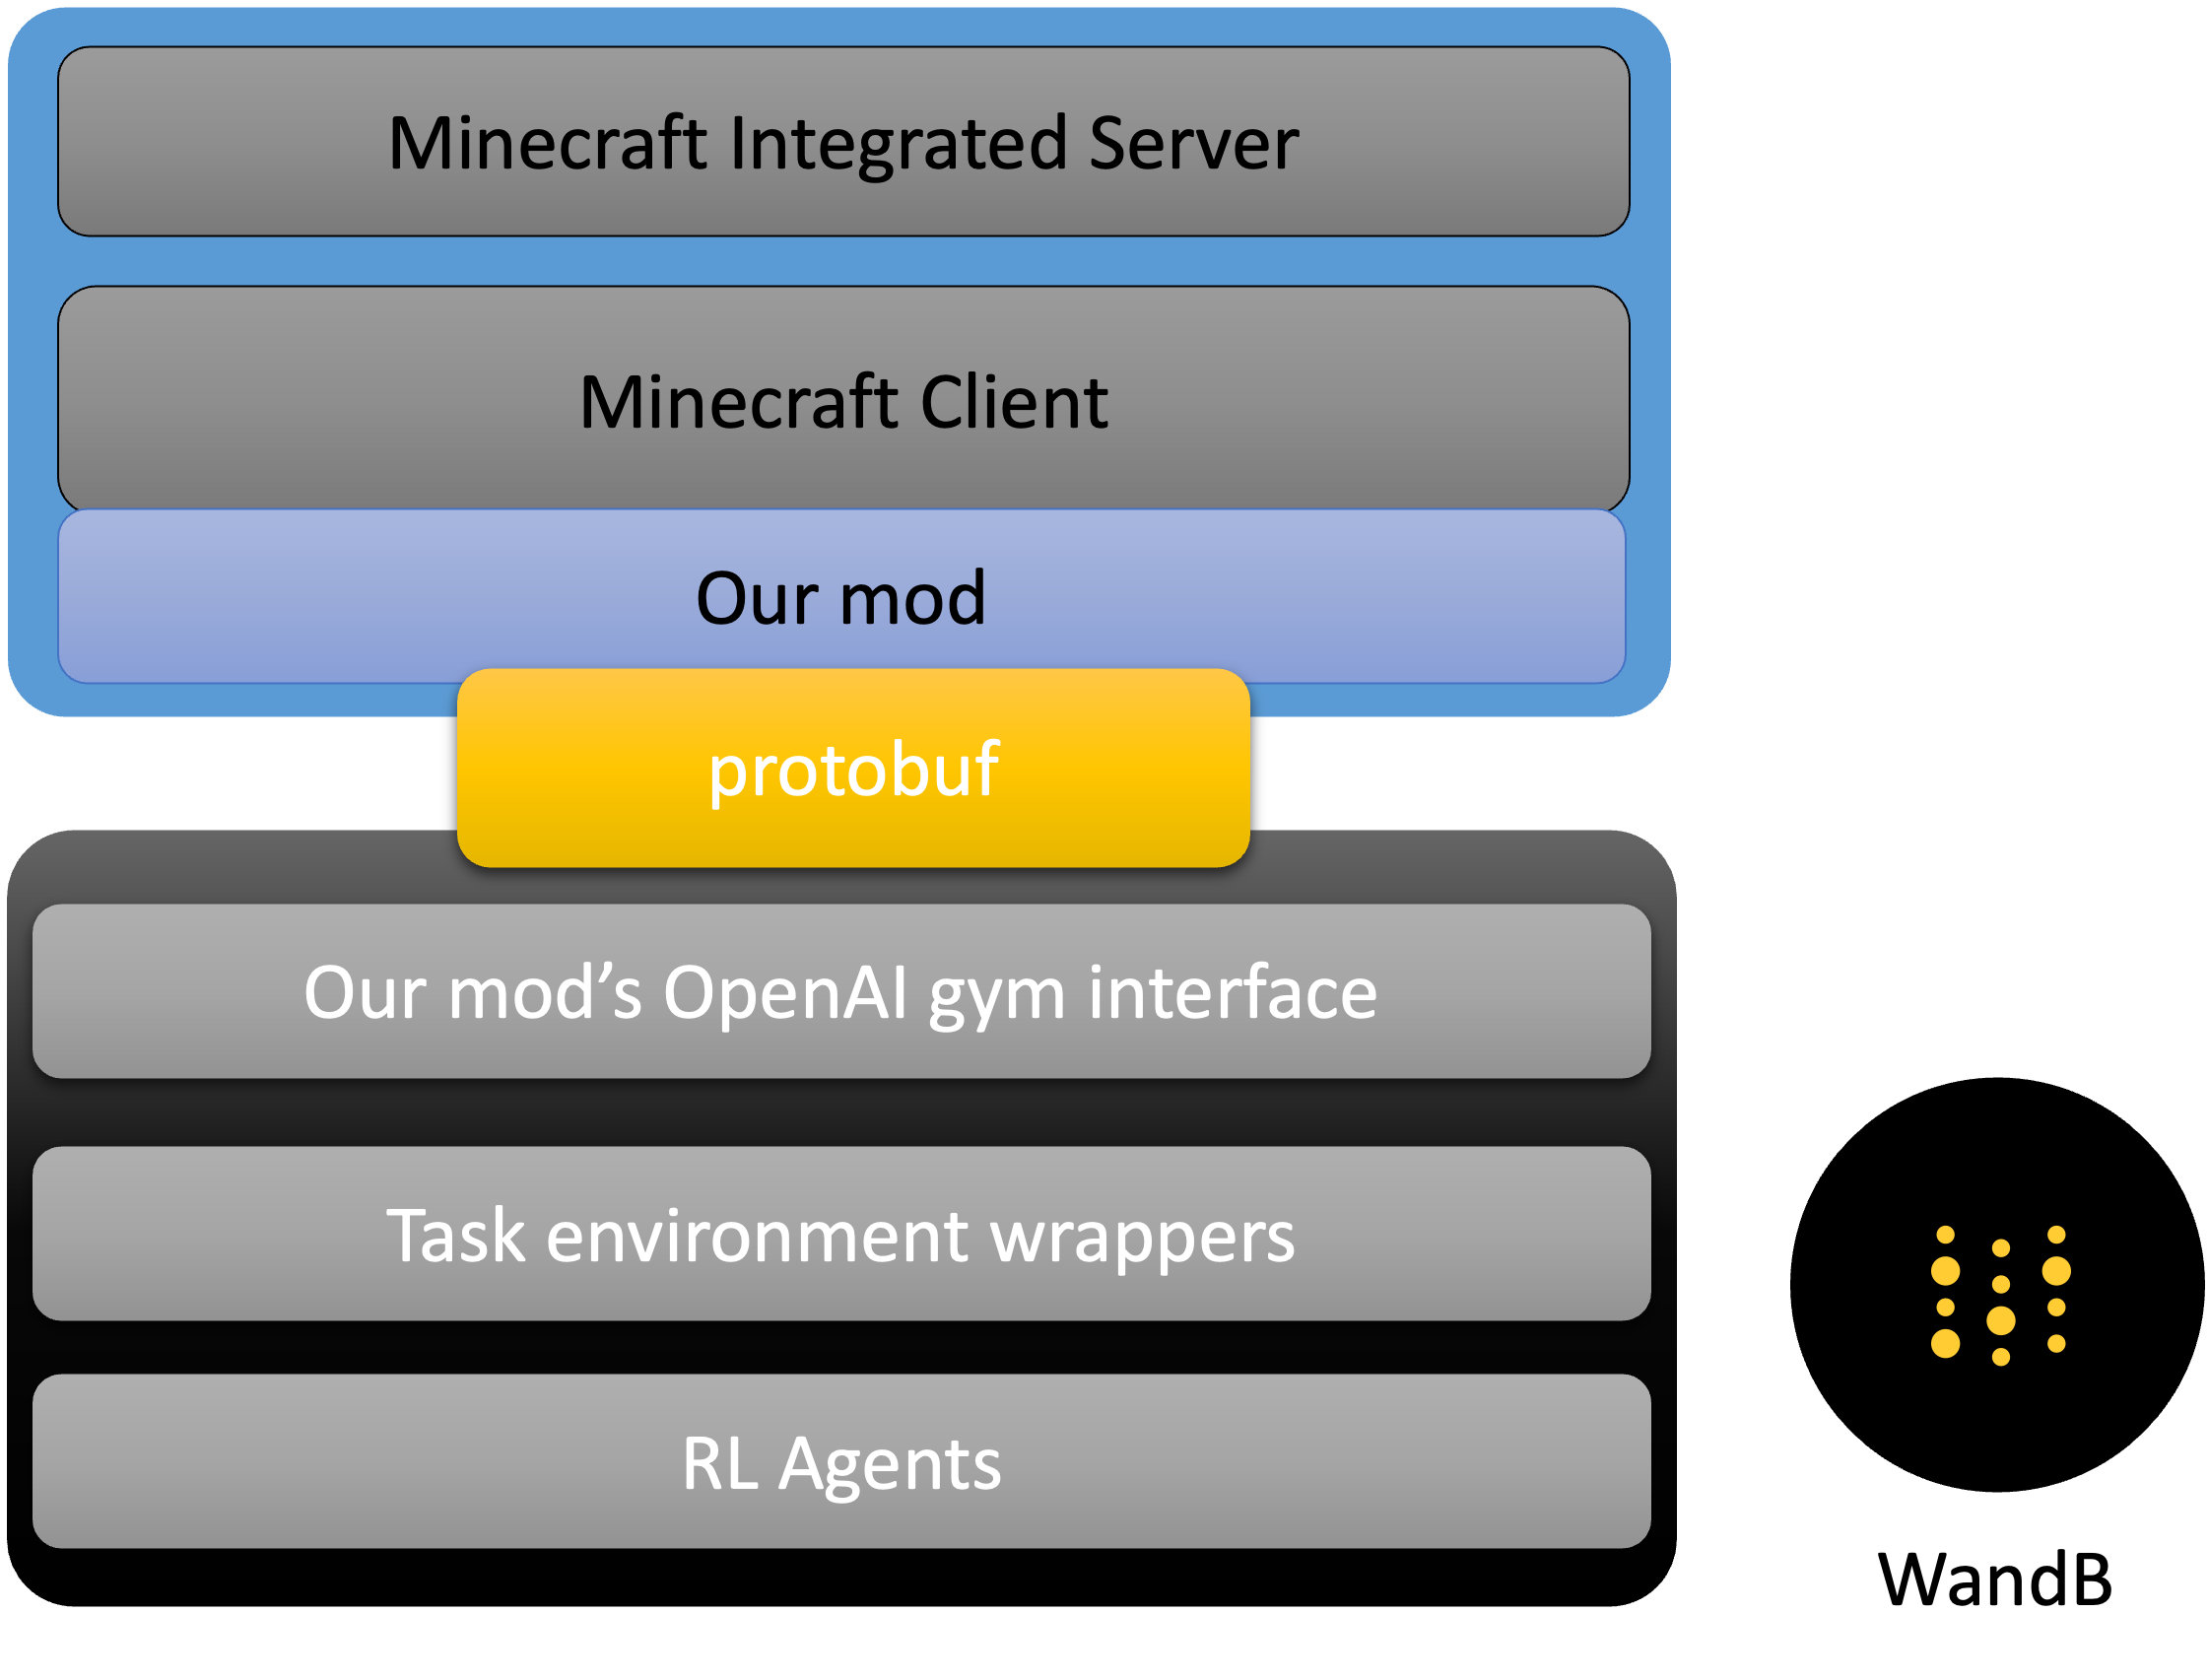
\includegraphics[width=.3\textwidth]{arch1.png}
  \caption{환경을 나타내는 그림. 강화학습 에이전트가 env.reset이나 step을 호출하면, 우리의 wrapper는 마인크래프트를 실행한 후, protobuf over TCP를 통해 우리의 마인크래프트 모드와 통신한다. 마인크래프트 모드는 플레이어를 조작하고, 관측 공간을 캡처하여 wrapper에게 전달한다. wrapper는 관측 공간을 처리하여 강화학습 에이전트에게 전달한다.}
  \label{fig:test}
\end{figure}

% \begin{tikzpicture}[node distance=3pt,
%   blueb/.style={
%     draw=white,
%     fill=mybluei,
%     rounded corners,
%     text width=2.5cm,
%     font={\sffamily\bfseries\color{white}},
%     align=center,
%     text height=12pt,
%     text depth=9pt},
%   greenb/.style={blueb,fill=mygreen},
%   ]
%   \node[blueb] (RCP) {RCP main};
%   \node[blueb,right=of RCP] (Aut) {Authoring};
%   \node[blueb,right=of Aut] (Bro) {Browsing};
%   \node[blueb,right=of Bro] (Pub) {Publishing};
%   \node[blueb,right=of Pub] (Sea) {Search};
%   \node[blueb,below=of RCP] (RTe) {Rich Text};
%   \node[blueb,right=of RTe,text width=5cm+10pt] (LMa) {Library Management};
%   \node[blueb,right=of LMa] (XML) {XML Export /\\[-0.7ex] Import};
%   \node[blueb,right=of XML] (MSP) {MSP Export};
%   \node[blueb,below=of RTe] (Com) {Common};
%   \node[blueb,right=of Com,text width=5cm+10pt] (UMA) {UMA};
%   \node[blueb,right=of UMA,text width=5cm+10pt] (EI) {Export/Import};
%   \node[blueb,below=of Com] (Jti) {Jtidy};
%   \node[greenb,right=of Jti,text width=5cm+10pt] (EMF) {EMF};
%   \node[greenb,right=of EMF] (GEF) {GEF};
%   \node[greenb,right=of GEF] (ICU) {ICUJ4};
%   \node[greenb,below=3.4cm of Bro,text width=13cm+26pt] (RCP) {RCP Runtime};
%   \begin{pgfonlayer}{background}
%   \draw[blueb,draw=black,fill=mybluei!30] 
%     ([xshift=-8pt,yshift=8pt]current bounding box.north west) rectangle 
%     ([xshift=8pt,yshift=-8pt]current bounding box.south east);
%   \end{pgfonlayer}
%   \node[blueb,draw=black,fill=myblueii,below=4.8cm of Bro,text width=13cm+44pt] (RCP) {RCP Runtime};
  
%   \end{tikzpicture}

% \begin{enumerate}
% \item 파이썬이 env.reset 수행
% \item gradle이 모드된 minecraft client를 실행
% \item minecraft client는 자동으로 주어진 조건에 맞추어 새로운 세계 생성
% \item minecraft client는 초기 상태를 python에 보냄
% \item python은 해당 정보를 가공하여 env.reset의 리턴값으로 삼음
% \item env.step에서 python은 조작 정보를 인코딩하여 minecraft client에 보냄
% \item minecraft client는 해당 정보를 바탕으로 플레이어를 조작
% \item 매 틱마다 클라이언트의 플레이어 조작 정보는 C2SPacket을 통해 서버에 보내짐
% \item 서버는 해당 정보를 바탕으로 해당 틱의 로직을 수행
% \item 클라이언트는 해당 틱이 끝나면 현재 화면을 캡처하고, 여러 obs 정보를 담아 python에 보냄
% \item 반복
% \end{enumerate}

\subsection{Tasks}
실험은 4개의 태스크와 3개의 모델을 이용하여 진행하였다. 먼저 태스크는 다음과 같다.
\begin{enumerate}
  \item 한 마리의 허스크를 피해 도망가기
  \item 여러 마리의 허스크를 피해 도망가기
  \item Darkness 상태 이상이 걸린 상태에서 한 마리의 허스크를 피해 도망가기
  \item 농장에서 동물 찾아가기
\end{enumerate}
3개의 모델은 다음과 같다.
\begin{enumerate}
  \item 시각 정보를 받는 CNN을 이용한 (D)DQN
  \item 소리와 방향 정보를 받는 Fully Connected Network를 이용한 (D)DQN
  \item 1과 2를 둘 다 이용하는 (D)DQN
\end{enumerate}

\subsection{보상 설계}
허스크를 피해 도망가는 태스크의 경우, 매 틱마다 살아있을 경우 0.5의 보상, 죽었을 경우 -1의 보상을 부여하였다. 동물 찾아가기 태스크의 경우, 매 틱마다 지정한 동물이 있는 장소에 도달했을 경우 1의 보상, 그렇지 않을 경우 -0.05의 보상을 부여하였다.

\subsection{모델 설계}
\subsubsection{시각 정보를 이용하는 에이전트}
$114 \times 64 \times 3$의 이미지를 입력으로 받는 CNN을 이용하였다. CNN의 구조는 다음과 같다.
(CNN그림인데 구조 확정이 안남)
\subsubsection{소리와 방향 정보를 이용하는 에이전트}
마인크래프트에 존재하는 소리 자막 기능을 커스터마이징하여 현재 에이전트에 대한 소리의 상대 좌표와 종류를 알아낼 수 있다. 상대 좌표 벡터를 정규화하고, 현재 에이전트가 바라보고 있는 yaw값은 trigonometric encoding을 하여 입력으로 주었다. 완전한 평지 지형에서 테스트하므로 y좌표는


\subsubsection{시각 정보와 소리, 방향 정보를 모두 이용하는 에이전트}



\section{연구 결과}

\subsection{구조도}
% \begin{figure}
%   \centering
%   \includegraphics[width=.3\textwidth]{result_revised}
%   \caption{연구 결과 시스템 개념도.}
%   \label{fig:result}
% \end{figure}


% \begin{figure}
%   \centering
%   \includegraphics[width=.35\textwidth]{block}
%   \caption{디바이스 드라이버가 메모장 실행을 차단한 모습. 메모장 프로세스는 생성되지 않으며, 메모장 실행이 차단되었다는 로그가 출력된다.}
%   \label{fig:block}
% \end{figure}

\subsection{연구 결과 소스 코드 저장소}
\href{https://github.com/KYHSGeekCode/MinecraftRL}{https://github.com/KYHSGeekCode/MinecraftRL}에서 본 포스터의 소스 코드를 탐색할 수 있다.

\section{한계점 및 논의}
\subsection{HTTPS}


\section{시사점}
이 연구는 타 분야에 비해 자료를 이해하기 어려운 DDK를 이용한 NT 레거시 윈도우 디바이스 개발이라는 분야에 유용한 예시를 제공하며, 이 연구를 통해 작성한 구현을 이용하여 비대면 강의 시 학생들의 집중을 도와주는 솔루션을 만드는 데 큰 도움을 준다는 데서 의의가 있다.
\bibliographystyle{unsrt}
\begin{thebibliography}{1}
    \bibitem{WDD2009}
    이봉석, 『윈도우 디바이스 드라이버』, {\em 한빛미디어}, 2009.
\end{thebibliography}


\end{document}
% vim: tw=80:ts=2:sts=2:sw=2:et:fdm=marker:fmr=[[[,]]]

